\chapter{Panel użytkownika niezarejestrowanego oraz niezalogowanego}

\section{Okno rejestracji użytkownika}
W poniższej sekcji ukazany zostanie interfejs programu umożliwiający użytkownikowi niezarejestrowanemu w systemie dokonania rejestracji. Rejestracja przebiegać może w~ dwóch wariantach:
\begin{itemize}
	\item Rejestracja przy użyciu konta \textit{Google},
	\item Rejestracja tradycyjna -- podanie adreu e-mail oraz hasła.
\end{itemize}

\subsection{Rejestracja przy użyciu konta \textit{Google}}
Opcja rejestracji i logowania za pomocą konta \textit{Google} znacznie ułatwia i przyspiesza proces dodawania nowego użytkownika. Pozwala ona zwiększyć odsetek nowych użytkowników systemu. Kolejnym powodem, który przemawia za tym, aby stosować logowanie przy użyciu danych pochodzących z portali społecznościowych jest fakt mówiący o tym, że adres e-mail, którym posługuje się dana osoba w momencie takiej rejestracji został już wcześniej zweryfikowany przez dostawcę sieci społecznościowej. Oznacza to, że w momencie logowania przy użyciu konta społecznościowego otrzymujemy rzetelne informacje, a~ nie fałszywe adresy, które użytkownicy wykorzystują zazwyczaj do zarejestrowania się na stronach internetowych. 

Cały proces rejestracji i pózniejszego logowania się do aplikacji przy użyciu konta \textit{Google} przebiega w następujący sposób: 
\begin{itemize}
	\item użytkownik wybiera opcję rejestracji w systemie i klika przycisk \textit{Zaloguj się za pomocą konta} \textit{Google} (rys. \ref{Rys:register}) i wpisuje dane logowania do konta \textit{Google}, bądź w~ przypadku kiedy jest zalogowany globalnie, wybiera odpowiednie konto (rys. \ref{Rys:choose_google}),
	\item żądanie rejestracji/logowania wysyłane jest do dostawcy sieci społecznościowej \textit{Google},
	\item w momencie gdy dostawca sieci społecznościowej \textit{Google} potwierdzi tożsamość użytkownika, bieżący użytkownik uzyskuje dostęp do aplikacji.
\end{itemize}

\newpage

\begin{figure}[h]
	\centering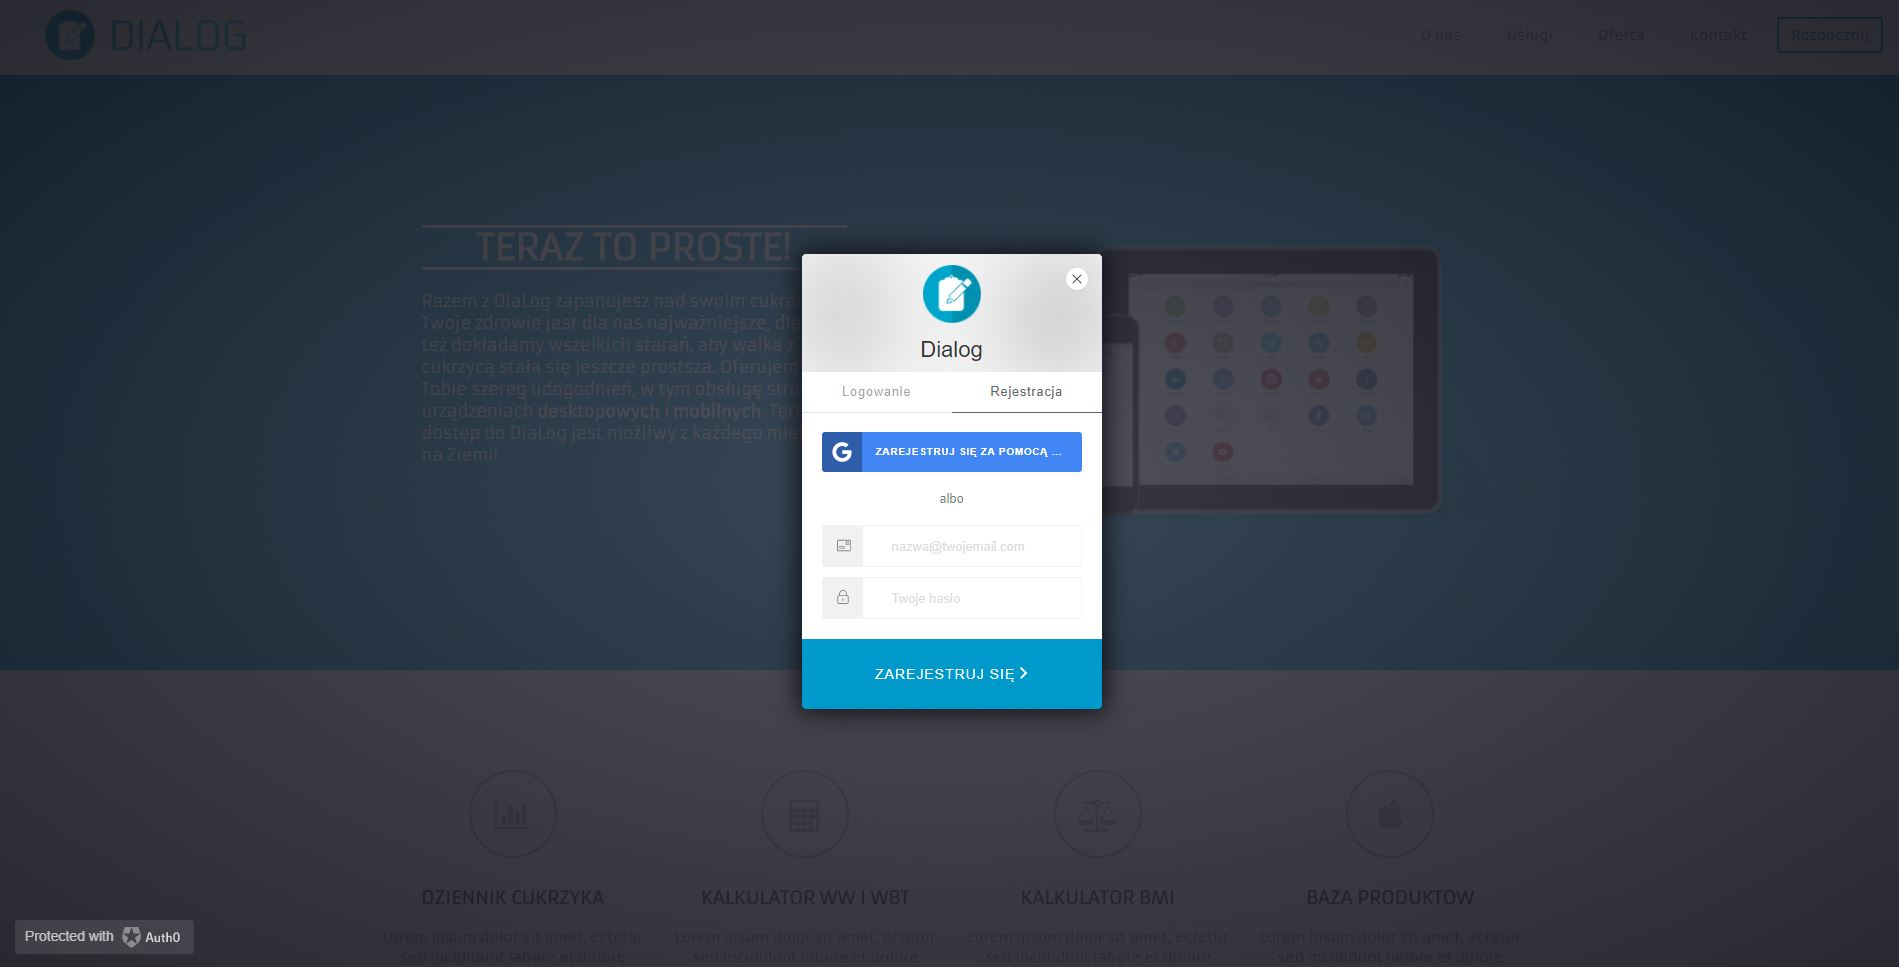
\includegraphics[scale=0.3]{images/register.jpg}
	\caption{Okno rejestracji użytkownika do systemu}
	\label{Rys:register}
\end{figure}

\begin{figure}[h]
	\centering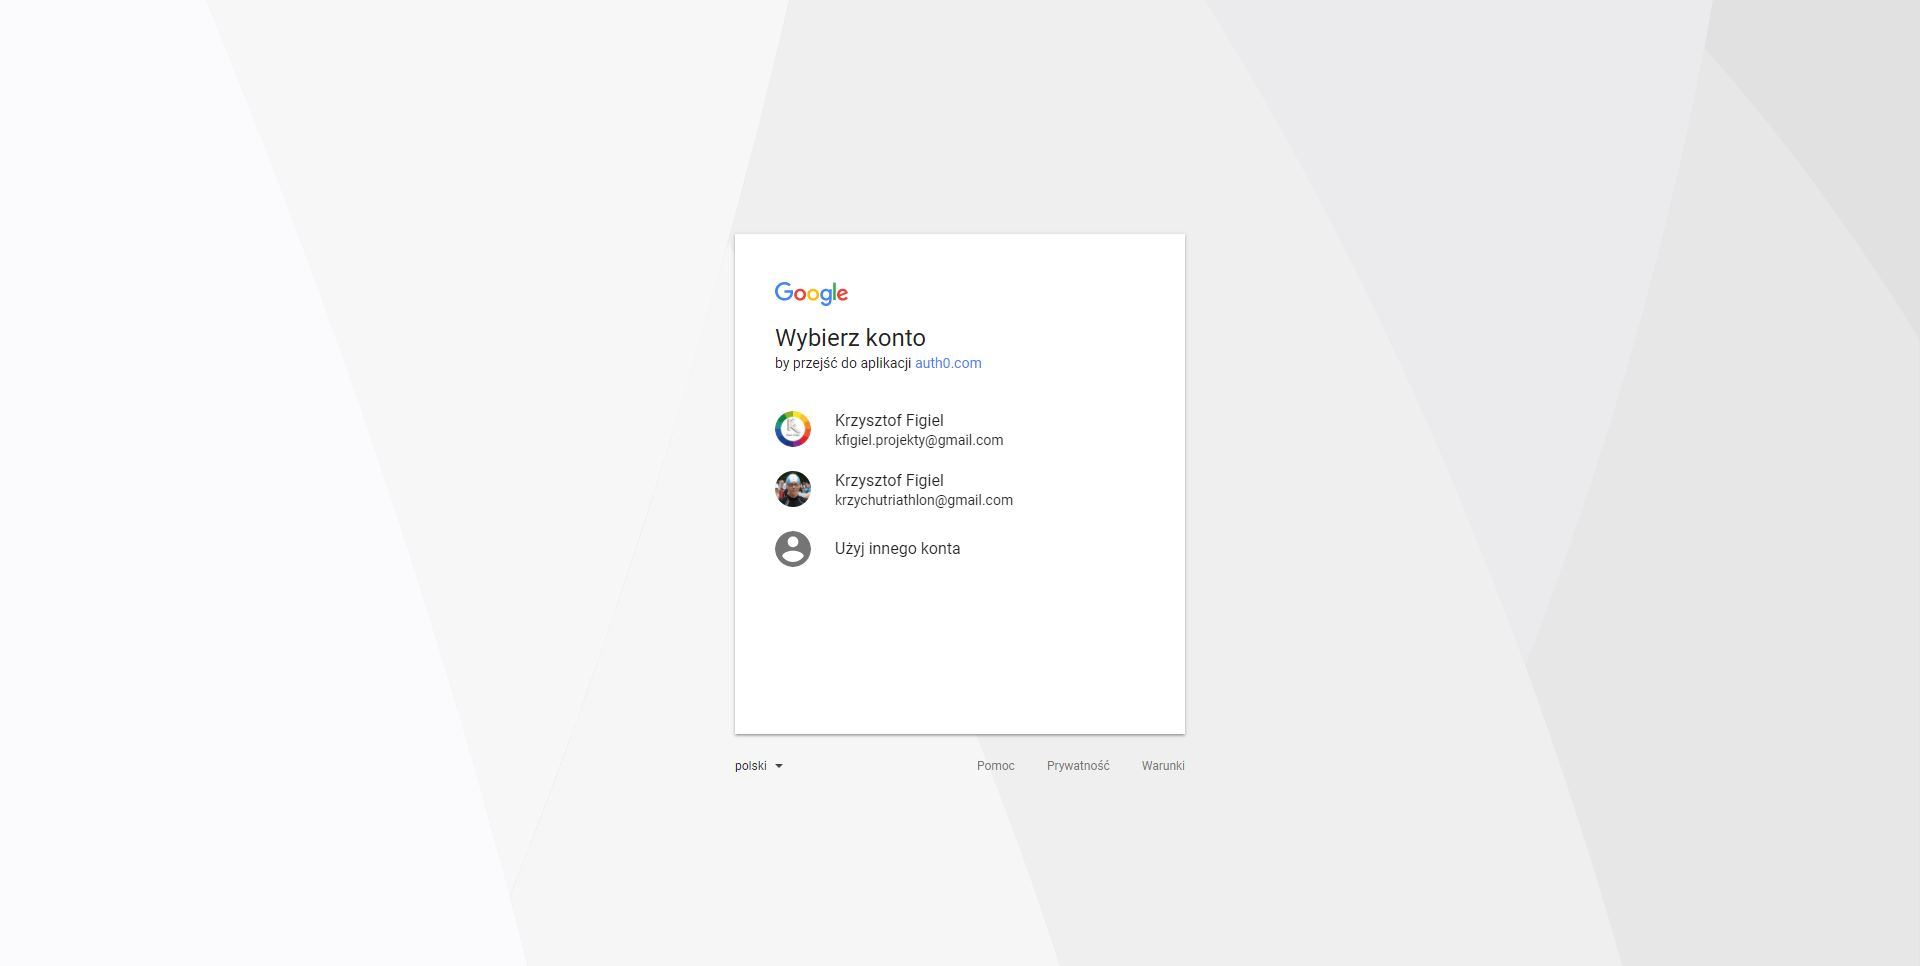
\includegraphics[scale=0.3]{images/google_account.jpg}
	\caption{Okno wyboru konta \textit{Google}}
	\label{Rys:choose_google}
\end{figure}

\subsection{Rejestracja tradycyjna -- podanie adreu e-mail oraz hasła}
W przypadku rejestracji tradycyjnej dane podane przez użytkownika (adres e-mail oraz hasło) zostają zapisane w zewnętrznej bazie danych dostawcy usług autoryzacji -- \textit{Auth0}. Po kliknięciu przycisku \textit{Zarejestruj się} (rys. \ref{Rys:normal_registration}) użytkownik zostaje powiadomiony o~ konieczności potwierdzenia autentyczności konta poprzez kliknięcie w link aktywacyjny wysłany automatycznie w wiadomości e-mail przez serwis \textit{Auth0} (rys. \ref{Rys:email_notification}). Po kliknięciu w link aktywacyjny możliwe jest już zalogowanie się. 

\newpage

\begin{figure}[h]
	\centering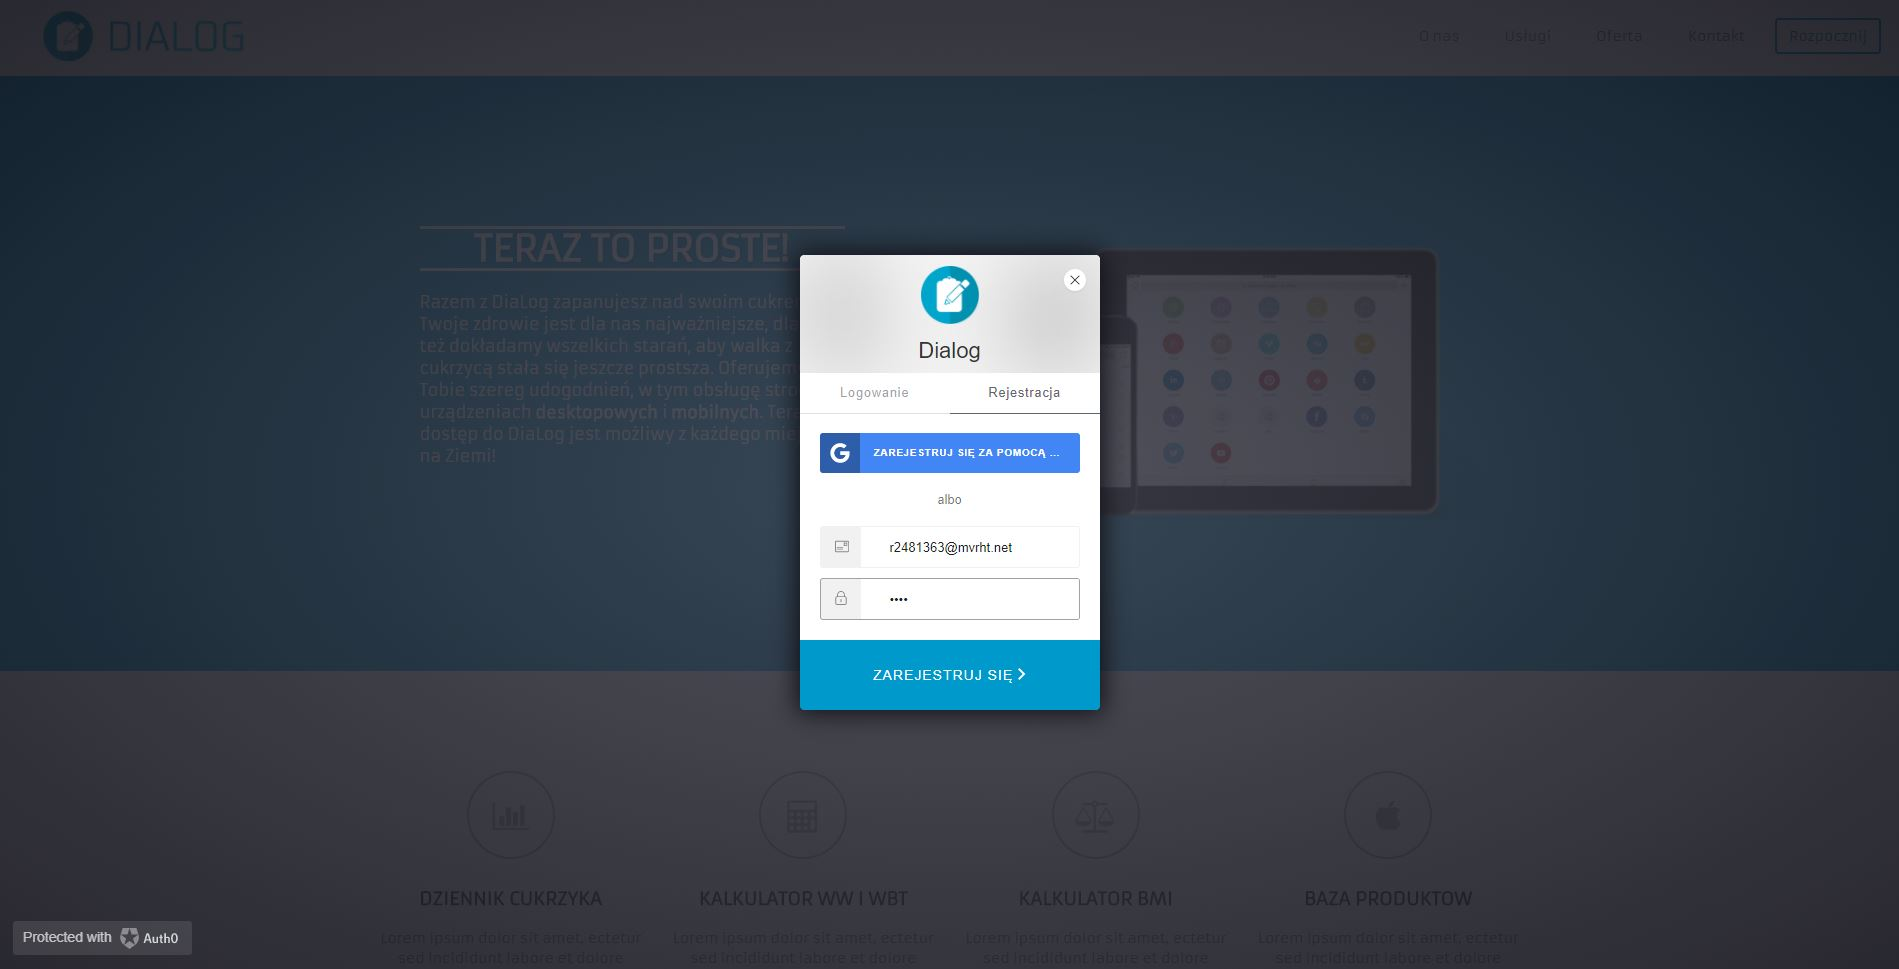
\includegraphics[scale=0.3]{images/normal_registration.jpg}
	\caption{Okno rejestracji tradycyjnej}
	\label{Rys:normal_registration}
\end{figure}

\begin{figure}[h]
	\centering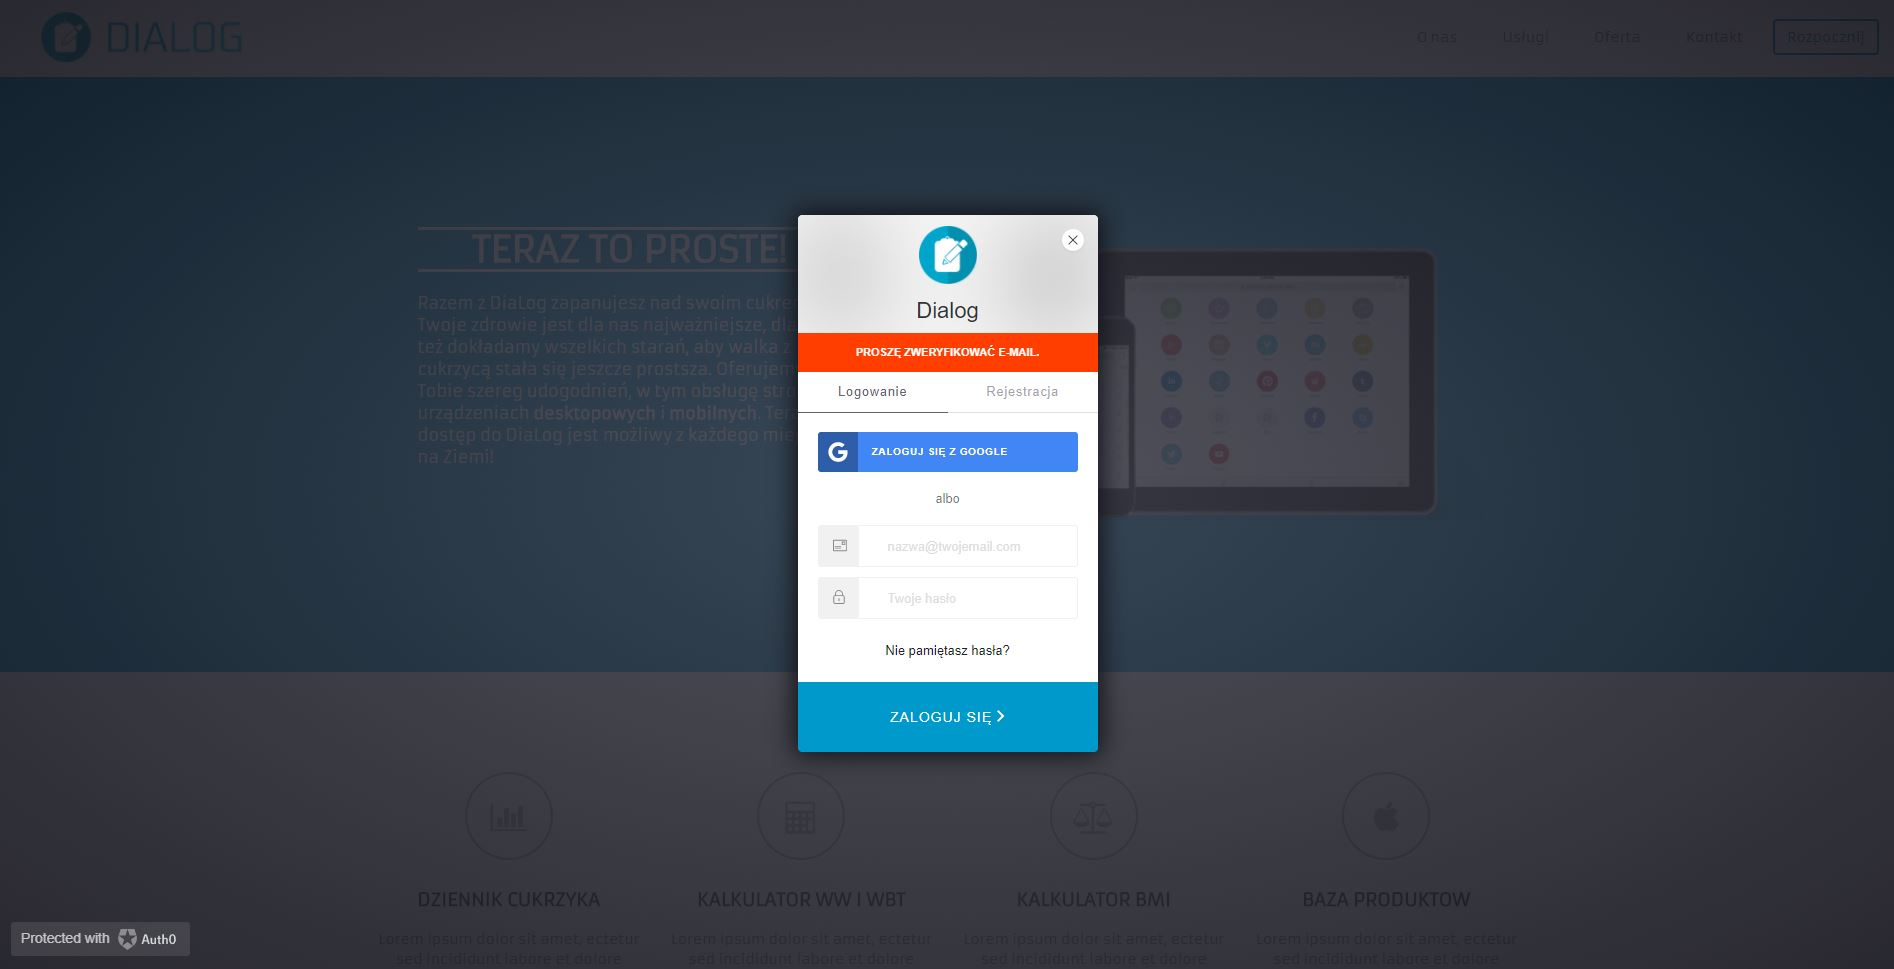
\includegraphics[scale=0.3]{images/email_verify.jpg}
	\caption{Okno z prośbą o potwierdzenie adresu e-mail}
	\label{Rys:email_notification}
\end{figure}

Po poprawnej rejestracji i późniejszym zalogowaniu się użytkownik ma dostęp do panelu użytkownika zarejestrowanego. Z poziomu panelu użytkownika niezalogowanego możliwe jest również uzyskanie informacji na temat funkcjonalności strony oraz wysłanie maila z zapytaniem do administracji za pomocą wbudowanego formularza z podpiętym modułem do wysyłania wiadomości e-mail. 

\newpage

Użytkownik może w każdej chwili wypełnić wymagane pola oraz wysłać wiadomość do administracji z dowolnym zapytaniem, klikając przycisk \textit{Wyślij} (rys. \ref{Rys:email_module}):
\begin{itemize}
	\item Imię,
	\item Nazwisko,
	\item Temat,
	\item Wiadomość
\end{itemize}

\begin{figure}[h]
	\centering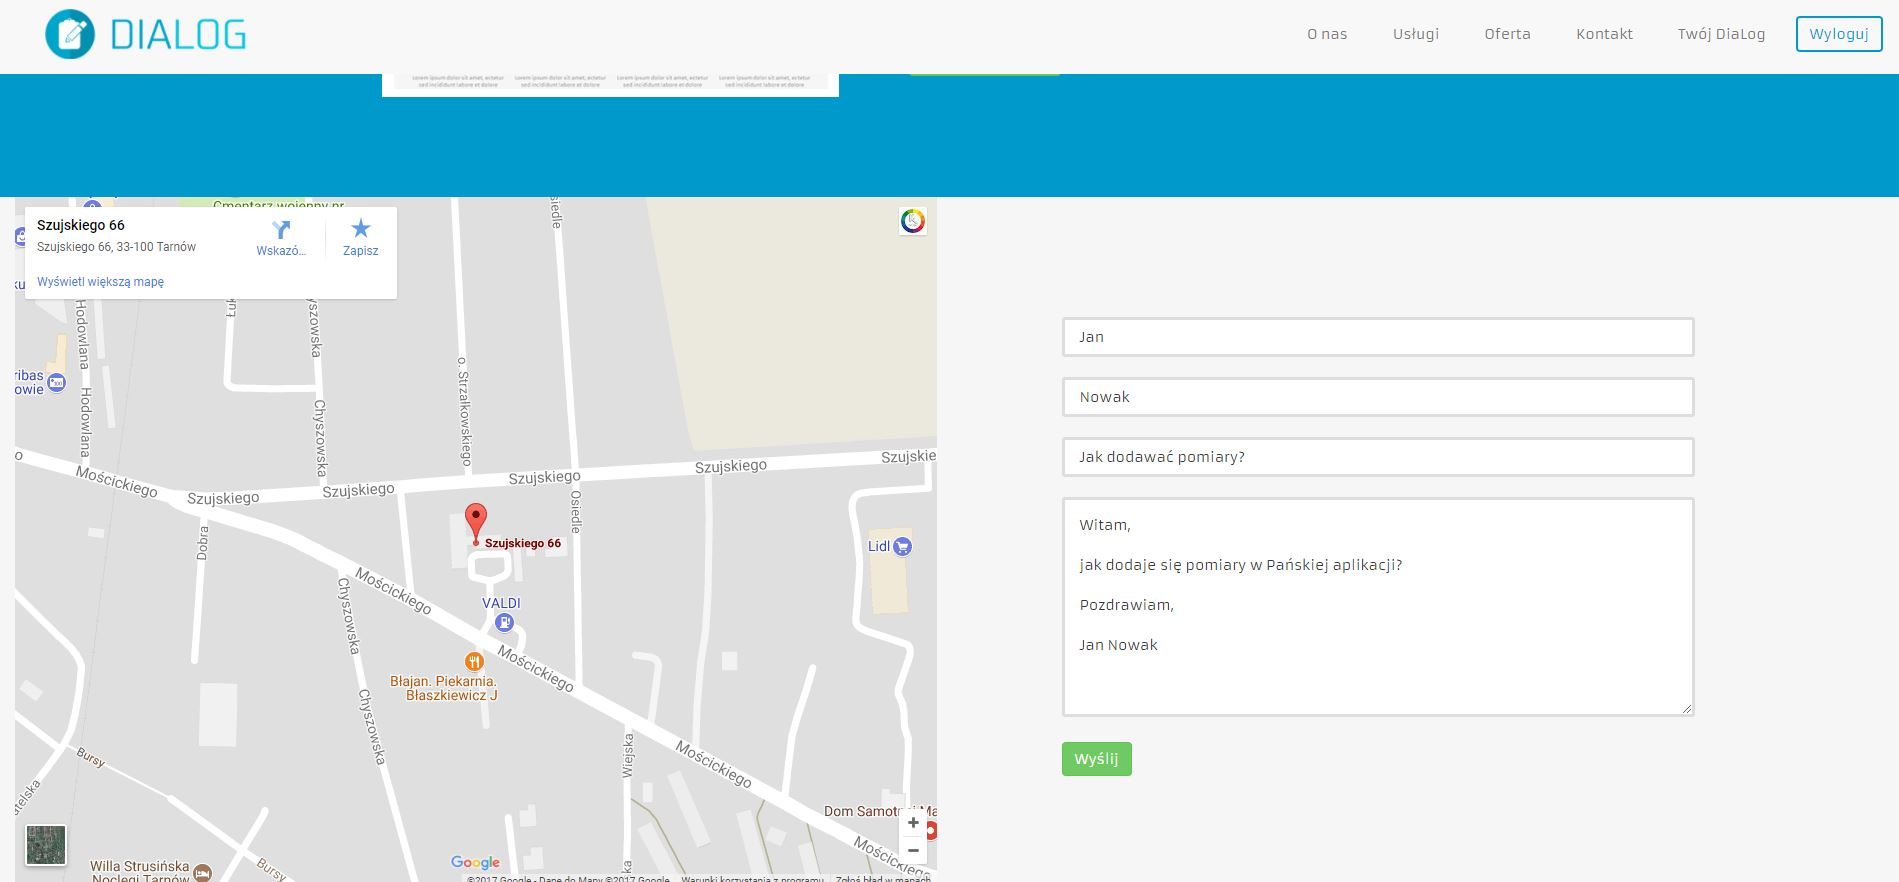
\includegraphics[scale=0.3]{images/email_module.jpg}
	\caption{Formularz do wysyłania maili do administracji}
	\label{Rys:email_module}
\end{figure}

